%%%%%%%%%%%%%%%%%%%%%%%%%%%%%%%%%%%%%%%%%%%%%%%%%%%%%%%%%%%%%%%%%%%%%%%%%%
% SwitchOnBehaviorAndSwitchOffBehaviorOfUI
%%%%%%%%%%%%%%%%%%%%%%%%%%%%%%%%%%%%%%%%%%%%%%%%%%%%%%%%%%%%%%%%%%%%%%%%%%

    \begin{figure}[ht]
        \centering
        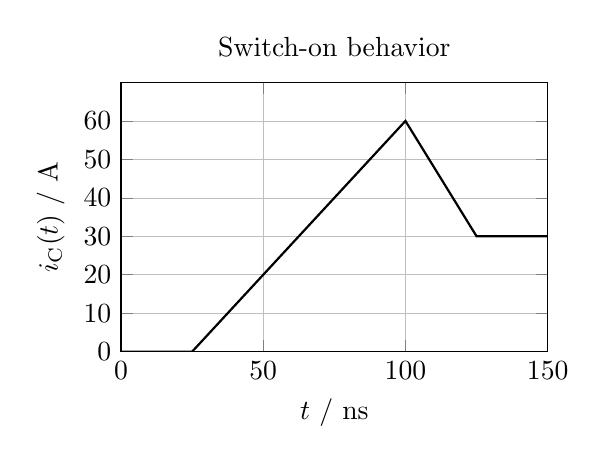
\begin{tikzpicture}
        \begin{axis}[
            width=7cm, height=5cm,
            grid=both,
            major grid style={line width=.2pt,draw=gray!50},
            minor grid style={line width=.1pt,draw=gray!20},
            xlabel={$t$ / ns},
            ylabel={$i_\mathrm{C}(t)$ / A},
            title={Switch-on behavior},
            xmin=0, xmax=150,
            ymin=0, ymax=70,
            xtick={0, 50, 100, 150},
            ytick={0, 10, 20, 30, 40, 50, 60},
            ]
            % Einschaltverhalten graph
            \addplot[
                thick,
                mark=none,
                color=black,
            ] coordinates {
                (0,0) (25,0) (50, 20) (75, 40) (100, 60) (125, 30) (150, 30)
            };
        \end{axis}
        \end{tikzpicture} 
        \hspace{1cm} % Abstand zwischen den beiden Diagrammen
        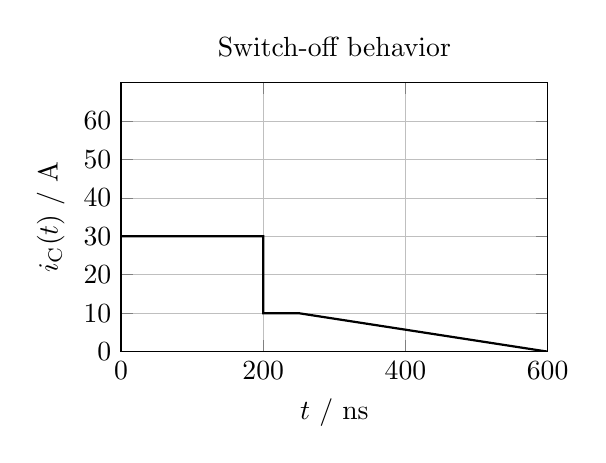
\begin{tikzpicture}
        \begin{axis}[
            width=7cm, height=5cm,
            grid=both,
            major grid style={line width=.2pt,draw=gray!50},
            minor grid style={line width=.1pt,draw=gray!20},
            xlabel={$t$ / ns},
            ylabel={$i_\mathrm{C}(t)$ / A},
            title={Switch-off behavior},
            xmin=0, xmax=600,
            ymin=0, ymax=70,
            xtick={0, 200, 400, 600},
            ytick={0, 10, 20, 30, 40, 50, 60},
            ]
            % Ausschaltverhalten graph
            \addplot[
                thick,
                mark=none,
                color=black,
            ] coordinates {
                (0,30) (200, 30) (200, 10) (250, 10) (600, 0)
            };
        \end{axis}
        \end{tikzpicture}
        \caption{Switch-on behavior and switch-off behavior of $i_{\mathrm{C}}(t)$}
        \label{fig:Switch-on behavior and switch-off behavior of}
    
        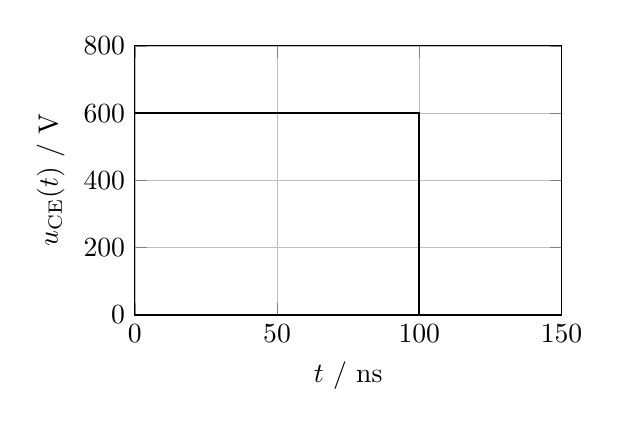
\begin{tikzpicture}
        \begin{axis}[
            width=7cm, height=5cm,
            grid=both,
            major grid style={line width=.2pt,draw=gray!50},
            minor grid style={line width=.1pt,draw=gray!20},
            xlabel={$t$ / ns},
            ylabel={$u_{\mathrm{CE}}(t)$ / V},
            xmin=0, xmax=150,
            ymin=0, ymax=800,
            xtick={0, 50, 100, 150},
            ytick={0,200, 400, 600, 800},
            ]
            % Einschaltverhalten graph
            \addplot[
                thick,
                mark=none,
                color=black,
            ] coordinates {
                (0,600) (100, 600) (100, 0)
            };
        \end{axis}
        \end{tikzpicture}
        \hspace{1cm} % Abstand zwischen den beiden Diagrammen
        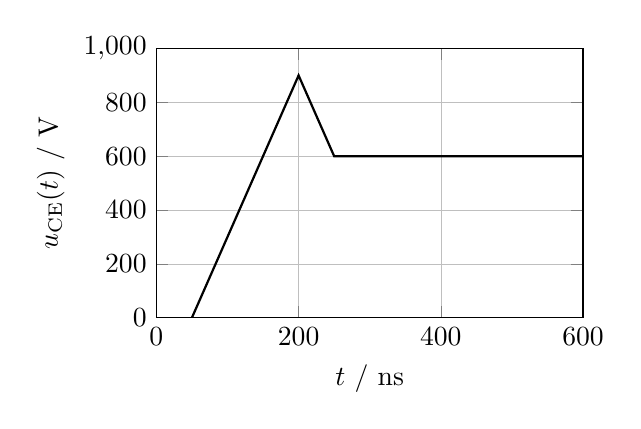
\begin{tikzpicture}
        \begin{axis}[
            width=7cm, height=5cm,
            grid=both,
            major grid style={line width=.2pt,draw=gray!50},
            minor grid style={line width=.1pt,draw=gray!20},
            xlabel={$t$ / ns},
            ylabel={$u_{\mathrm{CE}}(t)$ / V},
            xmin=0, xmax=600,
            ymin=0, ymax=1000,
            xtick={0,200, 400, 600},
            ytick={0,200, 400, 600,800, 1000},
            ]
            % Ausschaltverhalten graph
            \addplot[
                thick,
                mark=none,
                color=black,
            ] coordinates {
                (50,0) (200, 900) (250, 600) (600, 600)
            };
        \end{axis}
        \end{tikzpicture}
        \caption{Switch-on behavior and switch-off behavior of $u_{\mathrm{CE}}(t)$.}
        \label{fig:Switch-on behavior and switch-off behavior of voltage}
    \end{figure}
